\documentclass[12pt,a4paper]{article}
\usepackage[utf8]{vietnam}
\usepackage{fontspec}
\setmainfont{Times New Roman}
\usepackage{indentfirst}
\usepackage{hyperref}
\usepackage{tikz}
\usepackage[left=2.64cm,right=2.54cm,top=2cm,bottom=2cm]{geometry}
\usepackage{geometry}
\usepackage{array}
\usepackage{color}
\usepackage{wallpaper}
\setcounter{page}{2}
\makeatletter
\definecolor{dkgreen}{rgb}{0,0.6,0}
\definecolor{gray}{rgb}{0.5,0.5,0.5}
\definecolor{mauve}{rgb}{0.58,0,0.82}
\usepackage{listings}
\pagenumbering{arabic}
\usepackage{fancyhdr}
\usepackage{lastpage}
\usepackage{minitoc}
\pagestyle{fancy}
\fancyhf{}
\rhead{21127511 Nguyễn Quốc Huy}
\lhead{Vật lý đại cương}
\rfoot{Trang \thepage \hspace{1pt}  \pageref{LastPage}}
\usepackage{multicol}
\setlength{\columnsep}{1cm}
\begin{document}
\thispagestyle{empty}
\begin{LARGE}
    \begin{center}{\underline{\color{red}{\bf NATIONAL UNIVERSITY OF HO CHI MINH CITY}}}
    \end{center}
\end{LARGE}
\vspace*{1cm}
\begin{center}{\Huge \color{green}\textbf{KHOA CÔNG NGHỆ THÔNG TIN}}
\end{center}
\ThisCenterWallPaper{1}{New_KHTN.jpg}
\vspace*{15cm}
\begin{center}{\Huge \color{cyan}\textbf{Nguyễn Quốc Huy - 21127511}}
\end{center}
\vspace*{1cm}
\begin{center}
    {\Huge \color{cyan}\textbf{{LỚP 21CLC02 - VẬT LÝ ĐẠI CƯƠNG}}}
\end{center}
\newpage
\let\cleardoublepage\clearpage

\tableofcontents

\newpage
\section{\textbf{\color{red}CHƯƠNG 4 : CƠ HỌC VẬT RẮN}}
\Large \subsection{\color{blue}\textbf{BÀI 1} }
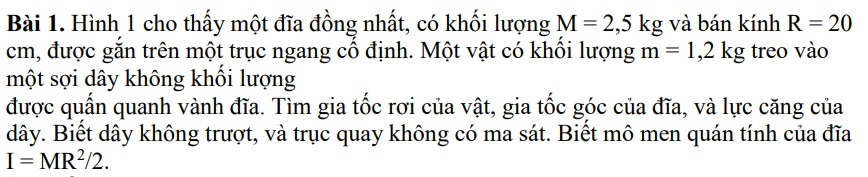
\includegraphics[scale=0.80]{N04_1.jpg}

\vspace*{1cm}
Áp dụng định luật II Newton :  Vật m = $ \vec{P} + \vec{T} = m\vec{a}$

\vspace*{1cm}
$\Leftrightarrow P - T = ma$ (*)

\vspace*{1cm}
Ta có : $ M = IB \Leftrightarrow T.R = IB \Leftrightarrow T.R = \frac{MR^2}{2} . \frac{a}{R}$

\vspace*{1cm}
$\Leftrightarrow T = \frac{Ma}{2}$

\vspace*{1cm}
$ mg - \frac{Ma}{2} = ma$
$\Leftrightarrow a = $ 
$\frac{Mg}{m + \frac{M}{2}} $
$\approx 4,8 (m/s^2)$

\vspace*{1cm}
Gia tốc : $B = \frac{a}{R} = 24 (rad/s^2)$

\vspace*{1cm}
Lực căng dây $T = \frac{Ma}{2} = 2,5 . 4,8 . 0,5 = 6(N)$

\newpage
\vspace*{1cm}
\Large \subsection{\color{blue}\textbf{BÀI 3} }
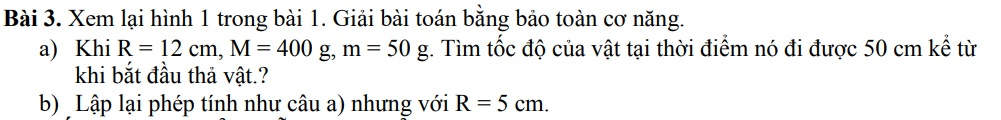
\includegraphics[scale=0.80]{No4_3.jpg}

\vspace*{1cm}
Chọn gốc thế năng tại vị trí ban đầu các vật, Áp dụng ĐL bảo toàn cơ năng:

\vspace*{1cm}
$\frac{mV^2}{2} - m.g.S + \frac{I\omega^2}{2} = 0$

\vspace*{1cm}
$\Leftrightarrow 0,025V^2 - 0,245+ \frac{1}{4}.0,4.V^2 = 0$ (V không phụ thuộc vào R)

\vspace*{1cm}
$ V = 1,4 (m/s^2)$

\vspace*{1cm}
Câu b/ Do V không phụ thuộc vào R nên với R thay đổi V luôn bằng $1,4 (m/s^2)$

\Large \subsection{\color{blue}\textbf{BÀI 4} }
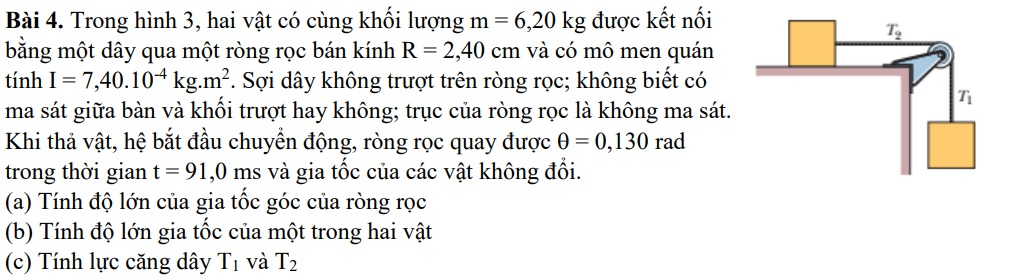
\includegraphics[scale=0.80]{No4_4.jpg}

\vspace*{1cm}
Ta có $\Delta\Omega =\frac{Bt^2}{2} \Leftrightarrow B = \frac{0,13 .2}{0,091} = 31,4 (rad/s^2)$

\vspace*{1cm}
$Gia tốc a = B.R = 0,754 (m/s^2)$

\vspace*{1cm}
Áp dụng định luật II Newton :  $Vật m_1 =  \vec{P} + \vec{T} = m\vec{a}$

\vspace*{1cm} Chiếu lên phương chuyển động : $P_1 - T_1 = m_1a$

\vspace*{1cm}
$\Rightarrow T_1 = 56,1 (N) $

\vspace*{1cm}
Phương trình chuyển động quay :

\vspace*{1cm}
$T_1.R - T_2.R = IB \Leftrightarrow (56,1 - T_2).0,024 = 7,4.10^{-4} .31,4$

\vspace*{1cm}
$\Rightarrow T_2 = 55,1 (N)$

\vspace*{1cm}
\Large \subsection{\color{blue}\textbf{BÀI 5} }
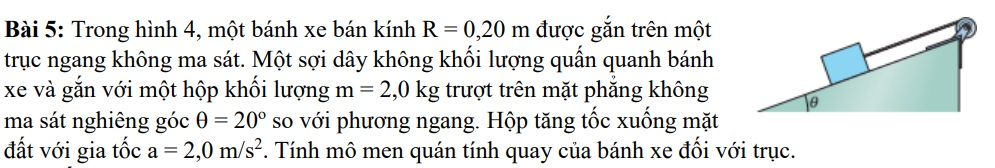
\includegraphics[scale=0.80]{No4_5.jpg}

\vspace*{1cm}
Áp dụng định luật II Newton: $ \vec{P} + \vec{T} = m\vec{a}$

\vspace*{1cm}
Chiếu lên chiều chuyển động : $\sin(20).P - T = ma$

\vspace*{1cm}
$ T = 2,7 (N)$

\vspace*{1cm}
Phương trình chuyển động quay : $ T.R = I.B$

\vspace*{1cm}
$\Leftrightarrow T.R = I. \frac{a}{R} \Leftrightarrow I = 0,054 (kg.m^2)$
\vspace*{1cm}
\Large \subsection{\color{blue}\textbf{BÀI 6} }

\includegraphics[scale=0.80]{No4_6.jpg}

\vspace*{1cm}
Áp dụng định lý động năng :

\vspace*{1cm}
$ E_2 - E_1 = A \Leftrightarrow 0 - (\frac{mV^2}{2} + \frac{I\omega^2}{2}) = A$

\vspace*{1cm}
$\Leftrightarrow -\frac{mV^2}{2} - \frac{mR^2}{2} . \frac{V^2}{R^2} = A$

\vspace*{1cm}
$\Leftrightarrow A = - mV^2 \Leftrightarrow A = -3,15 (J)$

\end{document}